\documentclass{amsart}
\usepackage{graphicx}     

\usepackage[hidelinks]{hyperref}
\usepackage{float}

\title{MIT 6.4400 Computer Graphics Final Project Check-in}
\author{David M. Berthiaume}

\date{\today}



\begin{document}



\maketitle

\begin{abstract}
This document summarizes my current progress with the final project for MIT 6.4400 Computer Graphics. 
\end{abstract}

\tableofcontents



\section{Project Summary}

The goal of this project is to create a ray tracer completely from scratch using Python and Numba and to render an artistic miniature planet based on real-world data.


\section{Progress Made}
The core ray tracer and algorithms to produce most of the geometry for the planet have been completed. 
The following lists the features that have been implemented.

\begin{itemize}

\item \emph{Gathering and processing data for Massachussets.} This was a lot of work, but it went relatively quickly. 
I gathered LiDAR data, building footprints, land cover data, land use data, tree cover data, and imperviousness data and created a framework to turn each of these (polygon or raster)
layers into a unified dataset. I then implemented a routine which for a given address clips these layers into a unified raster (EPSG:32619 projection) at a given resolution for sampling during the geometry and material construction of the planet. 
\item \emph{Creating a ray tracer from scratch.} I significantly underestimated how much work this was going to be, especially to make the ray-tracer performant enough to render 
tens of millions of triangles in under a minute at 2000x2000 resolution. 
  \begin{itemize}
      \item I implemented many of the standard algorithms for ray tracing including Phong lighting.
      \item The most difficult part was making it performant enough to handle tens of millions of geometries in a reasonable amount of time to allow for rapid iteration and debugging. Taking advantage of the 
the particular geometry of this scene, with its nearly spherical shape and symmetry, I implemented a custom octtree(ish) data structure that allows me to 
recursively perform axis-aligned bounding box intersections optimally to reduce the number of expensive intersections.
      \item In many areas of my rendering, I implemented perlin noise. This is used in the terrain, material types, and to the (spherical) background to make it more interesting.
  \end{itemize}
  \item \emph{Geometry generation.} I converted a projected set of data into two hemispheres and stitched them together. To accomplish this, I turned the heightmap into a mesh and then warped this into a hemisphere. I then mirrored this 
  mesh around the equator to create the 'dark side' of the planet. I place trees based on the tree cover layer and land cover types, and generate building geometries. I sample from the land use and land cover data layers to create custom materials for each location of the planet. For example, water is blue, reflective, and shiny. Certain elements are procedurally generated such as building heights and transitions from one land type to another.

\end{itemize}

\section{Challenges Faced and Next Steps}
Overall, this project has been \emph{significantly} more work than I expected it to be. 

Now that the core algorithms are implemented, I plan on implementing better lighting, shadows, reflections, artistic effects, and perhaps a simple asteroid ring around the center of the planet to help hide the obvious symmetry.

I wanted to do a live presentation, but I have a conflict with a final exam at Harvard. I will record a video instead.

\section{GitHub Repository}

I have made the GitHub repository for my ray tracer public. It can be found here: \url{https://github.com/davidberth/MITCGProject}.


\section{Screenshots of Current Progress}


\begin{figure}[H]
      \caption{A rendering of '236 Lake Ave Newton, MA 02460' (no shadows and only basic lighting implemented so far)}
      \begin{center}
            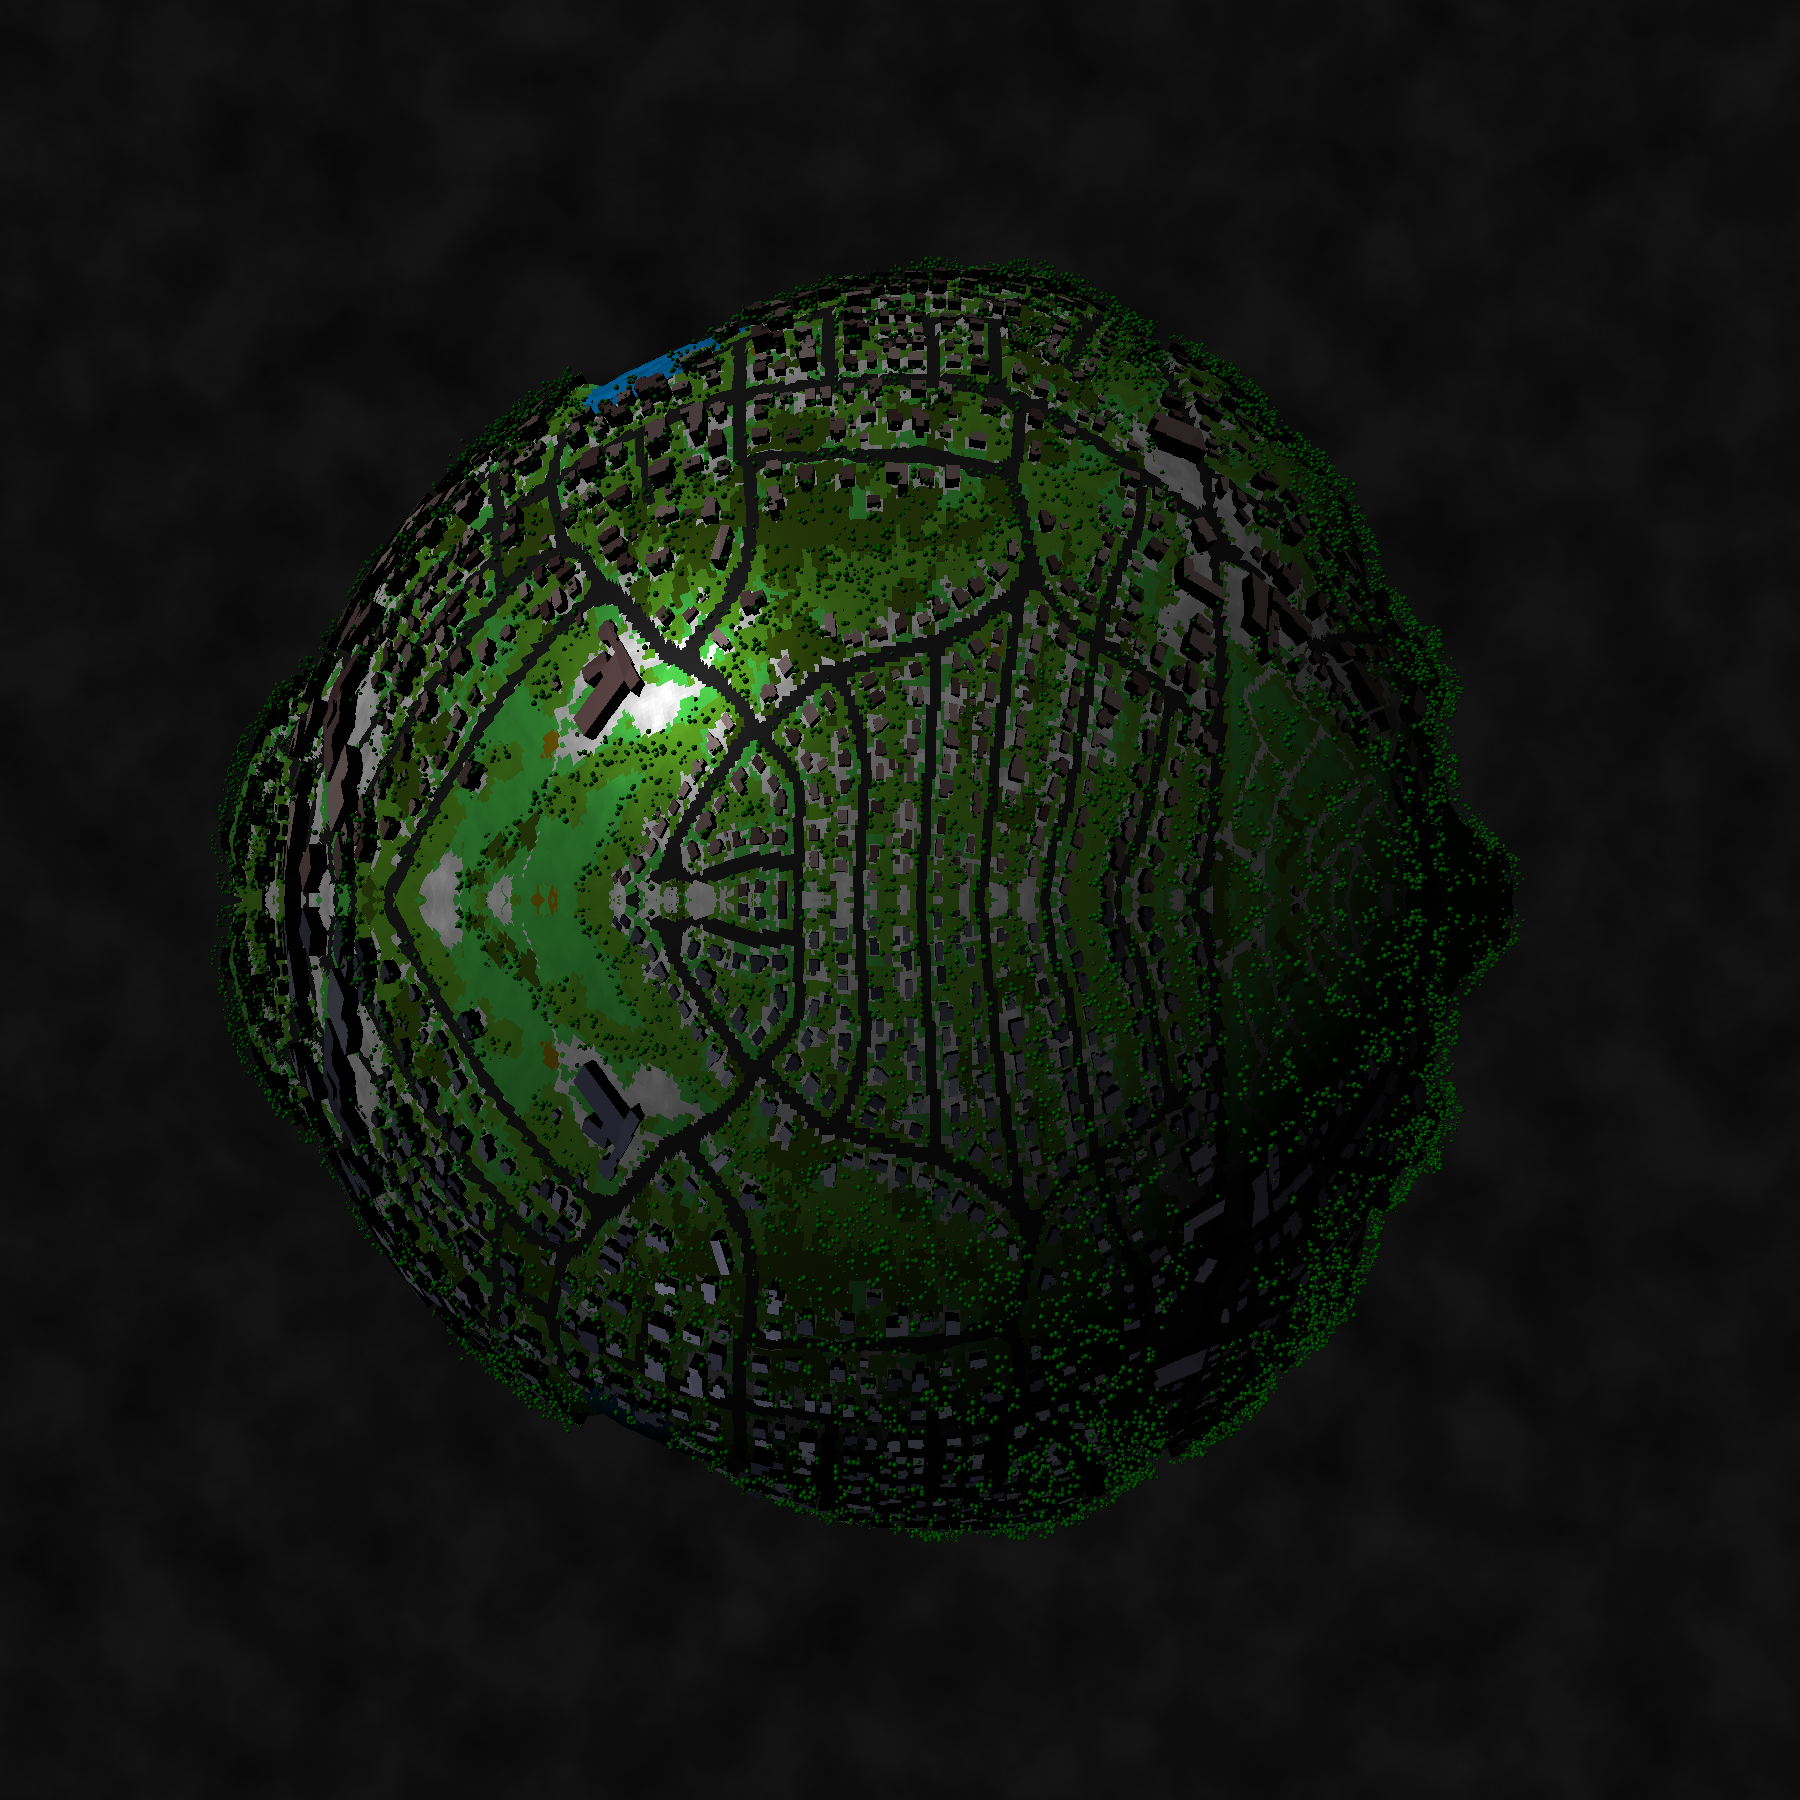
\includegraphics[width=5.5in]{../results/r1.png}
      \end{center}
\end{figure}

\begin{figure}[H]
      \caption{A rendering of '62 Jacqueline Rd, Waltham, MA 02452'}
      \begin{center}
            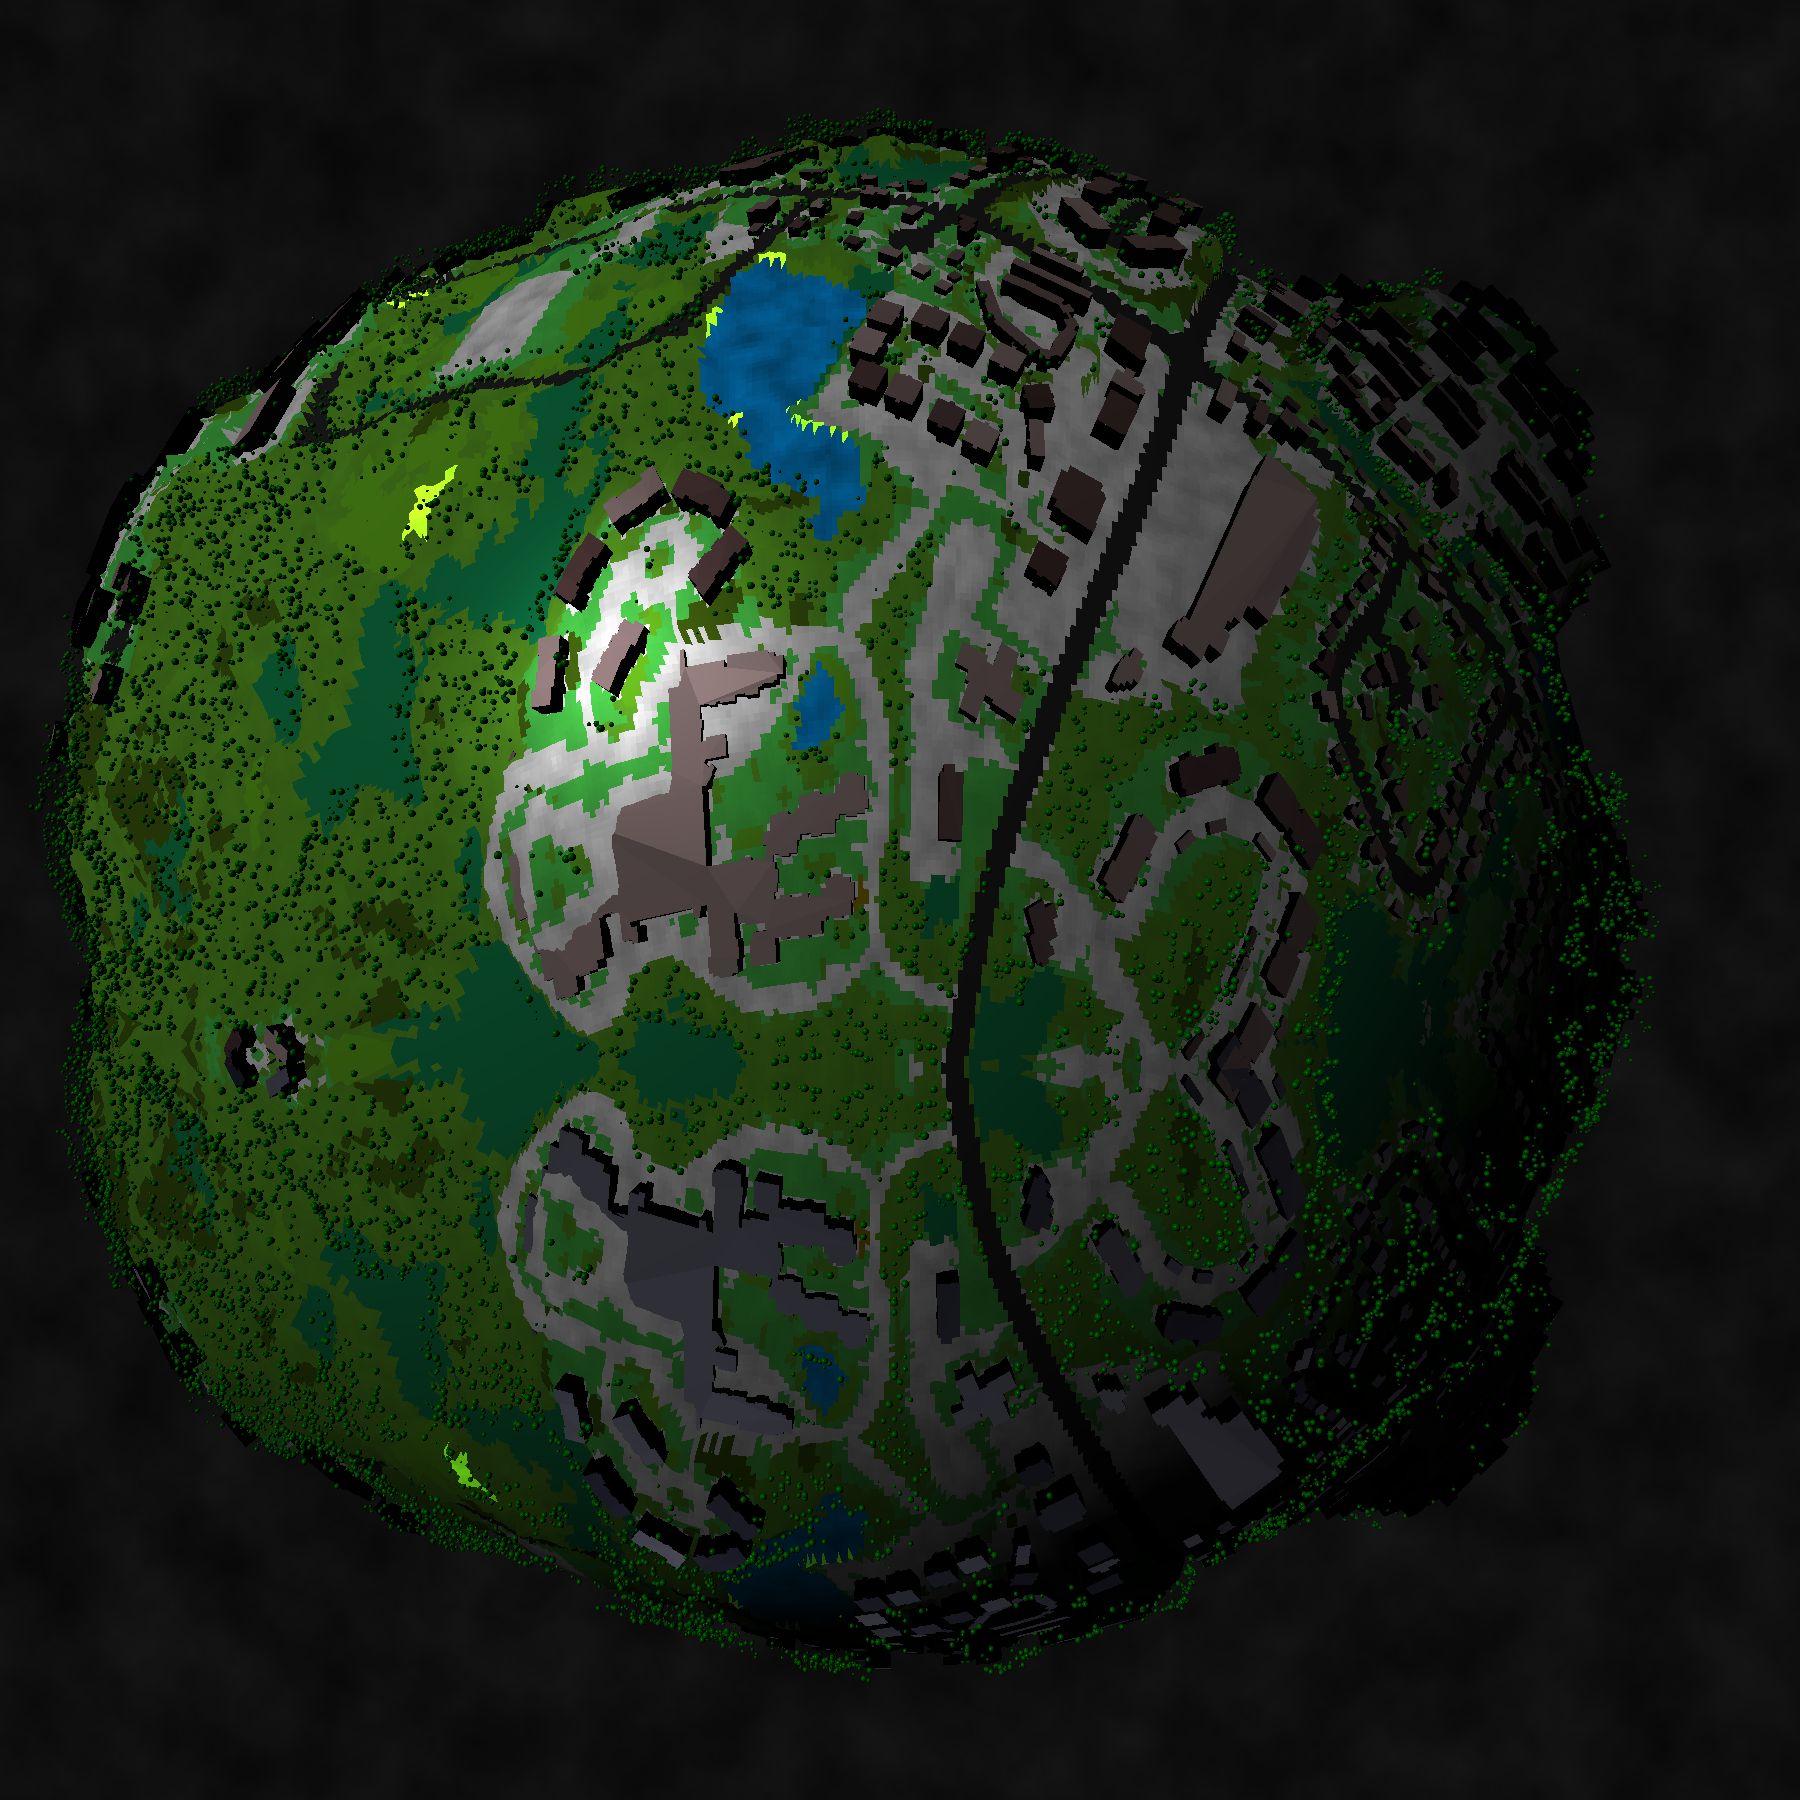
\includegraphics[width=4.5in]{../results/r2.png}
      \end{center}
\end{figure}

\begin{figure}[H]
      \caption{A rendering of a remote region in Spencer, MA}
      \begin{center}
            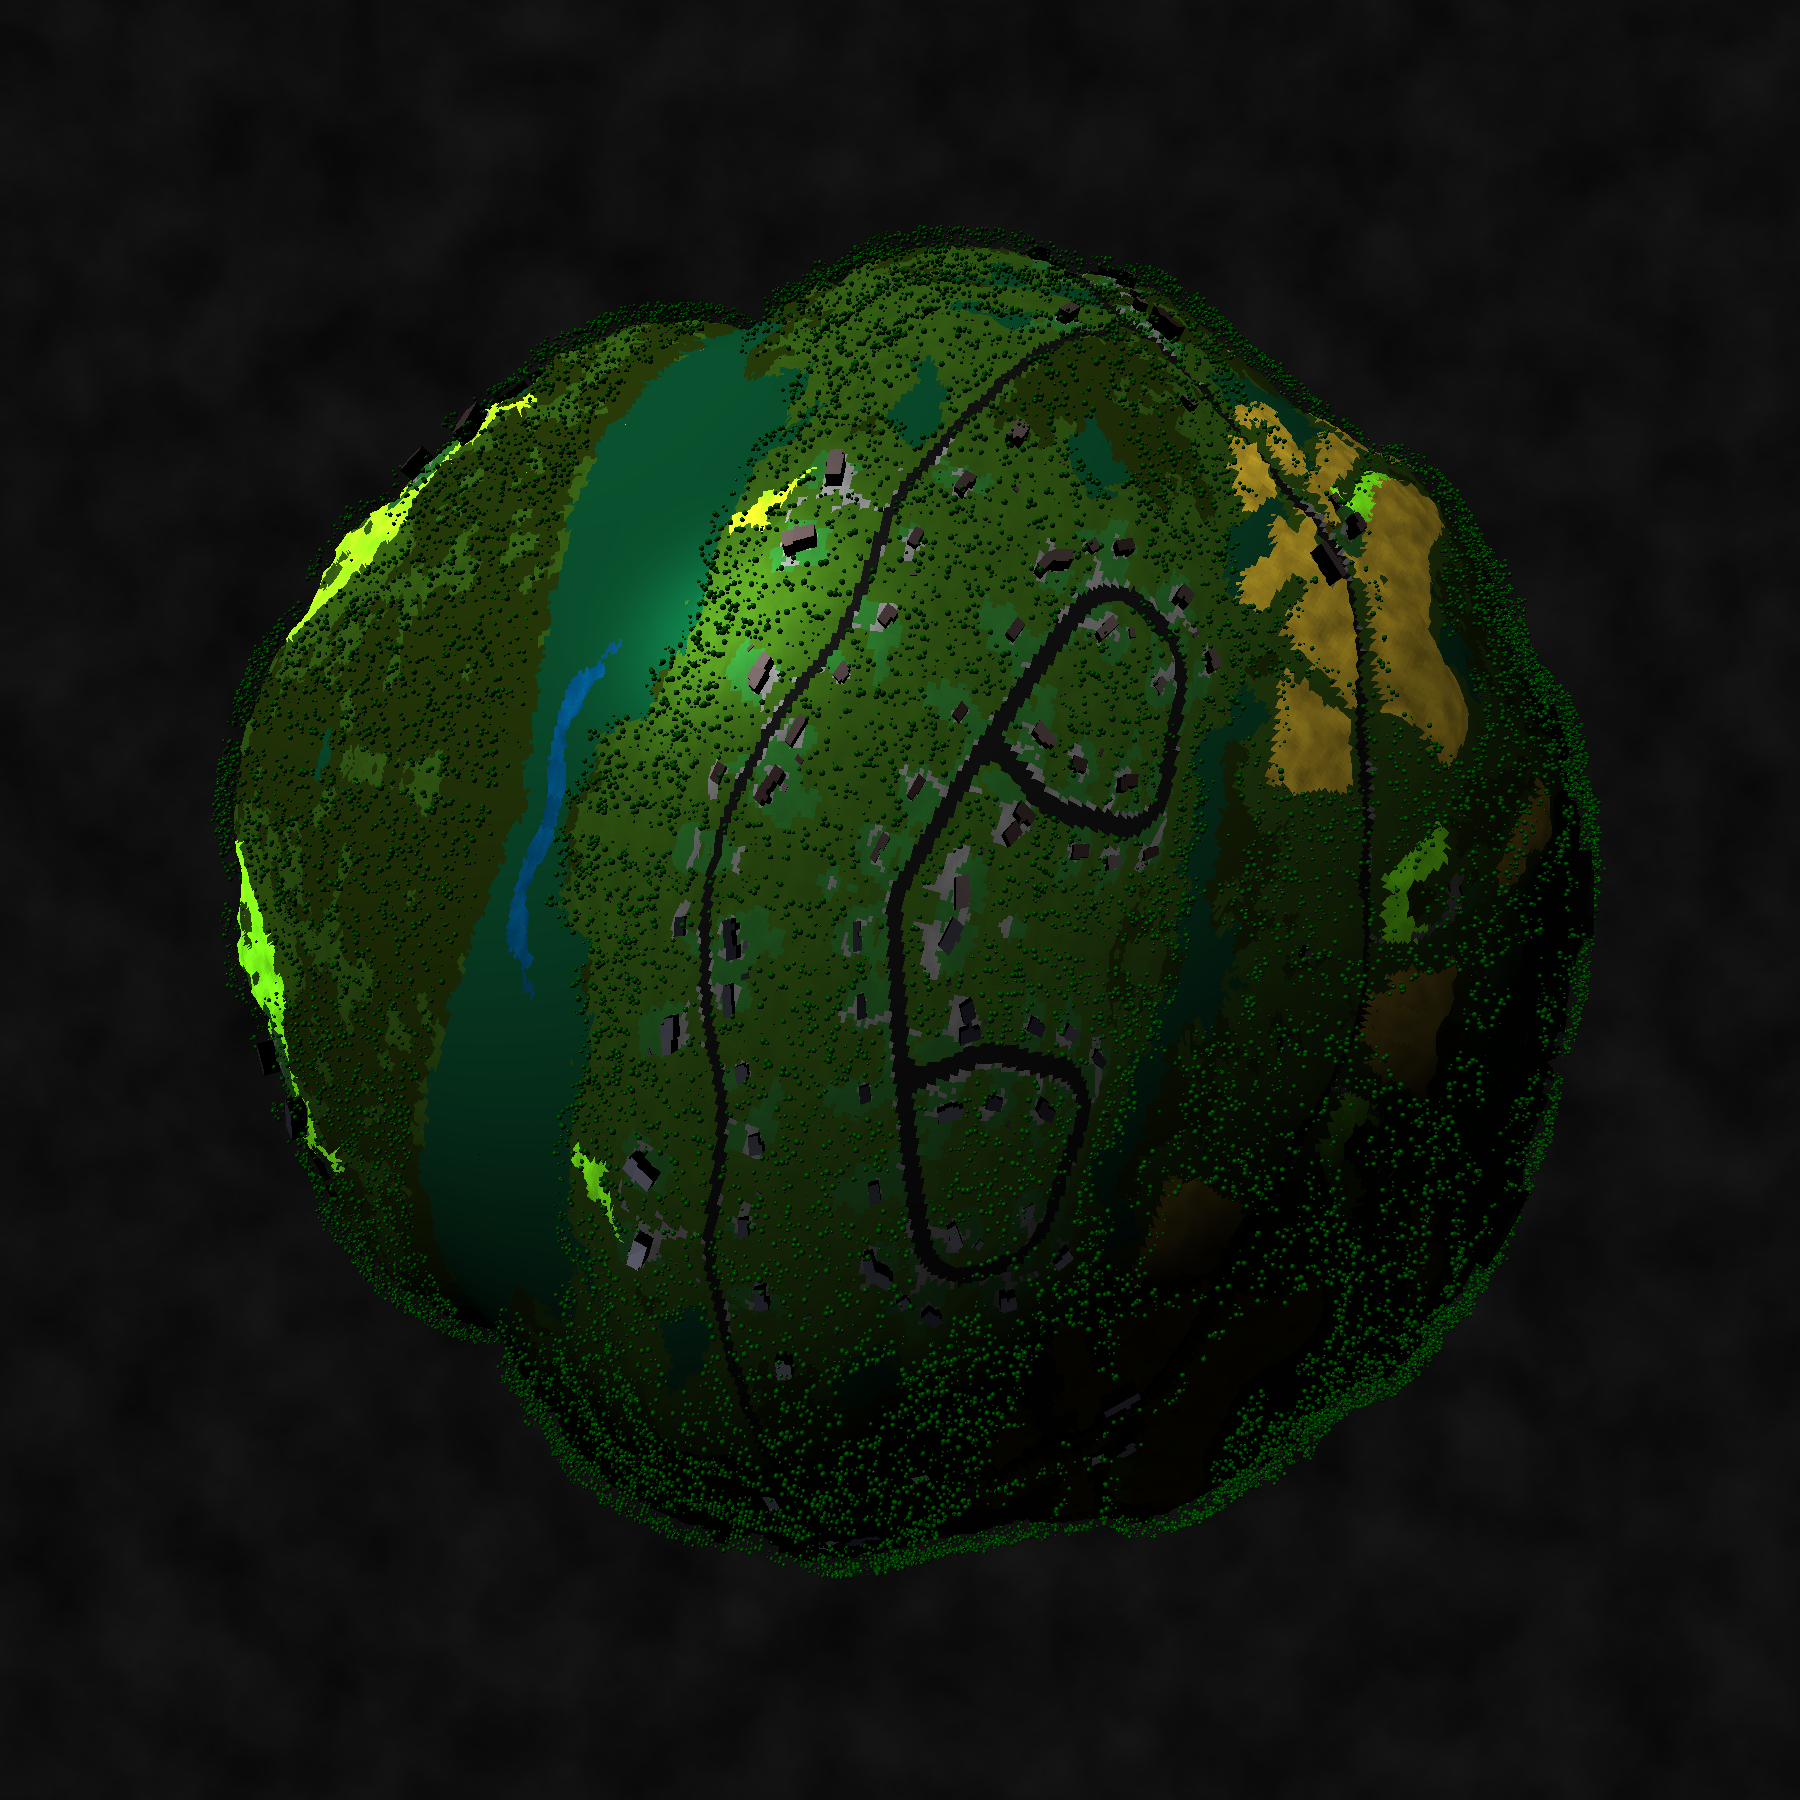
\includegraphics[width=4.5in]{../results/r3.png}
      \end{center}
\end{figure}


\section{Land Cover Types Implemented}

\begin{figure}[H]
      \caption{A list of land cover types that have been implemented so far}
      \begin{center}
            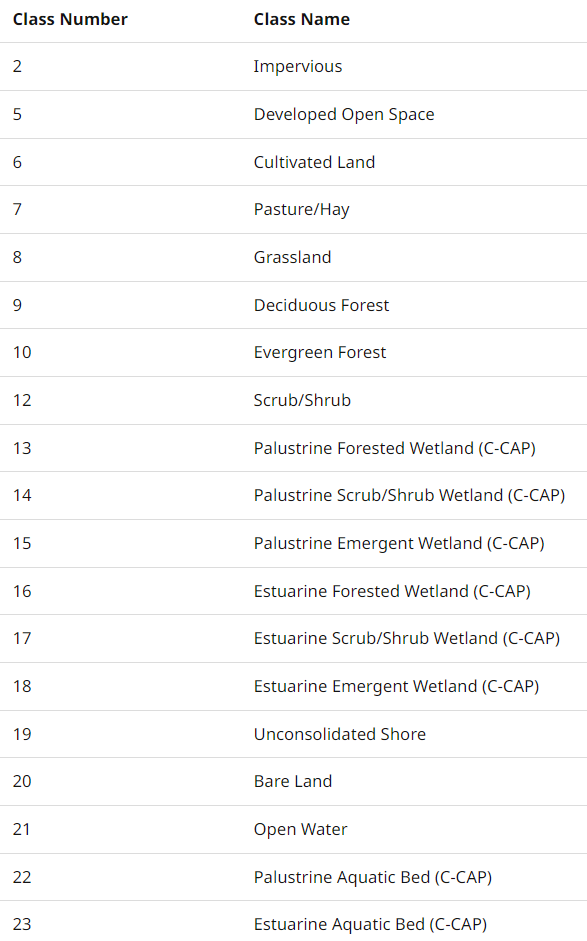
\includegraphics[width=4in]{../figures/landcover.png}
      \end{center}
\end{figure}


\section{References}

\begin{itemize}
      \item Book: The ray tracer challenge: a test-driven guide to your first 3D renderer Buck, Jamis (Access through Harvard library)

      \item MassGIS Bureau of Geographical Information

            \url{https://www.mass.gov/orgs/massgis-bureau-of-geographic-information}
      \item Ray tracing from scratch

            \url{https://raytracing.github.io/books/RayTracingInOneWeekend.html}
      \item Extracting 3D Bare-Earth Surface from Airborne LiDAR Data

            \url{https://ieeexplore.ieee.org/document/4562112} (Access through Harvard)
      \item Perlin noise generator for Python

            \url{https://pypi.org/project/perlin-noise/}
      \item Ray tracing and global illumination

            \url{https://digitalcommons.unf.edu/cgi/viewcontent.cgi?article=1100&context=ojii_volumes}

\end{itemize}



\end{document}